% -*- TeX-engine: xetex; eval: (auto-fill-mode 0); eval: (visual-line-mode 1); -*-
% Compile with XeLaTeX

\documentclass[11pt]{article}
%%%%%%%%%%%%%%%%
% Packages
%%%%%%%%%%%%%%%%

\usepackage[top=1cm,bottom=1cm,left=1.5cm,right= 1.5cm]{geometry}
\usepackage[parfill]{parskip}
\usepackage{graphicx, fontspec, xcolor,multicol, enumitem, setspace}
\DeclareGraphicsRule{.tif}{png}{.png}{`convert #1 `dirname #1`/`basename #1 .tif`.png}

%%%%%%%%%%%%%%%%
% No page number
%%%%%%%%%%%%%%%%

\pagestyle{empty}

%%%%%%%%%%%%%%%%
% User defined colors
%%%%%%%%%%%%%%%%

% Pantone 2015 Spring colors
% http://iwork3.us/2014/09/16/pantone-2015-spring-fashion-report/
% update each semester or year

\xdefinecolor{custom_blue}{rgb}{0, 0.70, 0.79} % scuba blue
\xdefinecolor{custom_darkBlue}{rgb}{0.11, 0.31, 0.54} % classic blue
\xdefinecolor{custom_orange}{rgb}{0.97, 0.57, 0.34} % tangerine
\xdefinecolor{custom_green}{rgb}{0.49, 0.81, 0.71} % lucite green
\xdefinecolor{custom_red}{rgb}{0.58, 0.32, 0.32} % marsala

\xdefinecolor{custom_lightGray}{rgb}{0.78, 0.80, 0.80} % glacier gray
\xdefinecolor{custom_darkGray}{rgb}{0.54, 0.52, 0.53} % titanium

%%%%%%%%%%%%%%%%
% Color text commands
%%%%%%%%%%%%%%%%

%orange
\newcommand{\orange}[1]{\textit{\textcolor{custom_orange}{#1}}}

% yellow
\newcommand{\yellow}[1]{\textit{\textcolor{yellow}{#1}}}

% blue
\newcommand{\blue}[1]{\textit{\textcolor{blue}{#1}}}

% green
\newcommand{\green}[1]{\textit{\textcolor{custom_green}{#1}}}

% red
\newcommand{\red}[1]{\textit{\textcolor{custom_red}{#1}}}

%%%%%%%%%%%%%%%%
% Coloring titles, links, etc.
%%%%%%%%%%%%%%%%

\usepackage{titlesec}
\titleformat{\section}
{\color{custom_blue}\normalfont\Large\bfseries}
{\color{custom_blue}\thesection}{1em}{}
\titleformat{\subsection}
{\color{custom_blue}\normalfont}
{\color{custom_blue}\thesubsection}{1em}{}

\newcommand{\ttl}[1]{ \textsc{{\LARGE \textbf{{\color{custom_blue} #1} } }}}

\newcommand{\tl}[1]{ \textsc{{\large \textbf{{\color{custom_blue} #1} } }}}

\usepackage[colorlinks=false,pdfborder={0 0 0},urlcolor= custom_orange,colorlinks=true,linkcolor= custom_orange, citecolor= custom_orange,backref=true]{hyperref}

%%%%%%%%%%%%%%%%
% Instructions box
%%%%%%%%%%%%%%%%

\newcommand{\inst}[1]{
\colorbox{custom_blue!20!white!50}{\parbox{\textwidth}{
	\vskip10pt
	\leftskip10pt \rightskip10pt
	#1
	\vskip10pt
}}
\vskip10pt
}

%%%%%%%%%%%%%%%%
% Timing
%%%%%%%%%%%%%%%%

% 15-20 minutes

%%%%%%%%%%%%%%%%
% Sakai link for course
%%%%%%%%%%%%%%%%

% UPDATE FOR OWN COURSE
% LINK TO ASSIGNMENTS TOOL IN SAKAI

\newcommand{\Sakai}[1]
{\href{https://sakai.duke.edu/portal/site/ba0d1c18-ba55-473f-9d70-b6a1f9559bbe/page/9870858b-a1a9-481e-8497-8a6ffe9e5be2}{Sakai}}

%%%%%%%%%%%
% App Ex number    %
%%%%%%%%%%%

% DON'T FORGET TO UPDATE

\newcommand{\appno}[1]
{6.1}

%%%%%%%%%%%%%%
% Turn on/off solutions       %
%%%%%%%%%%%%%%

% Off
\newcommand{\soln}[1]{
\vskip5pt
}

%% On
%\newcommand{\soln}[1]{
%\textit{\textcolor{custom_darkGray}{#1}}
%}

%%%%%%%%%%%%%%%%
% Document
%%%%%%%%%%%%%%%%

\begin{document}
\fontspec[Ligatures=TeX]{Helvetica Neue Light}

Dr. \c{C}etinkaya-Rundel \hfill Data Analysis and Statistical Inference \\

\ttl{Application exercise \appno{}: \\
Linear model}

\inst{Submit your responses on \Sakai{}, under the appropriate assignment. Only one submission per team is required. One team will be randomly selected and their responses will be discussed.}

\section*{Murders and poverty}

We want to build a model for for predicting annual murders per million from percentage living in poverty in a random sample of 20 metropolitan areas. The scatterplot below shows the relationship between these variables, and the summary table contains all values you will need to construct the linear model.

\begin{multicols}{2}
\begin{center}
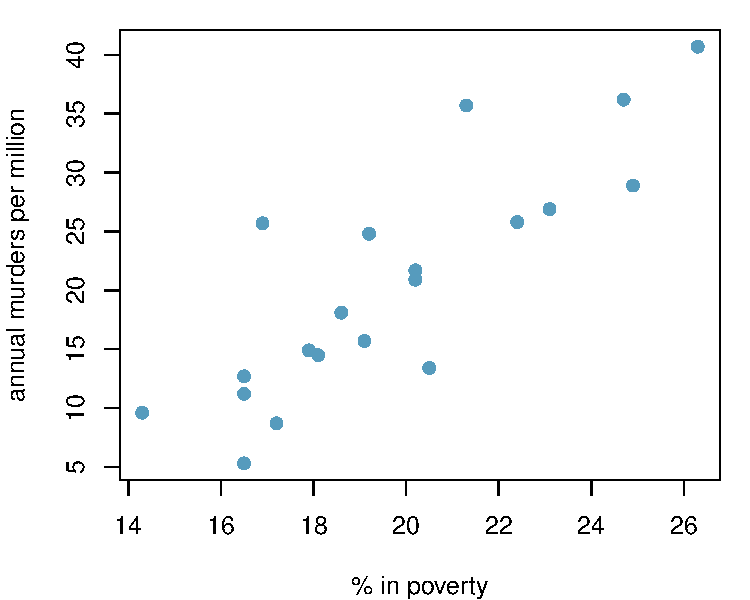
\includegraphics[width=0.4\textwidth]{murder/annual_murders_per_mil_perc_pov}
\end{center}
%
\begin{tabular}{l r r}
\hline
		& annual murders		& \% in poverty \\
		& / million $(y)$		& $(x)$   \\
\hline
mean	& $\bar{y} = 20.57$	& $\bar{x} = 19.72$  \\
sd		& $s_y = 9.88$		& $s_x = 3.24$ \\
\hline
		& correlation		& $R = 0.84$ \\
\hline
\end{tabular}
\end{multicols}
%

\begin{enumerate}

\item Calculate the slope.

\item Calculate the intercept.

\item Write out the linear model.

\end{enumerate}

\end{document}